Using the data available we were able to successfully rank the users on their relative influence compared to the selected group. In~\ref{eq:eigenvector} we only have 26 non-zero values in our approximated eigenvector. Our full results can be found in Appendix~\ref{app:results}

\begin{equation}\label{eq:eigenvector}
    \left\{
        \underbrace{%
            \begin{pmatrix}
                14\\
                21\\
                23\\
                32\\
                33\\
                34\\
                42\\
                52\\
                53\\
                57\\
                61\\
                65\\
                68\\
                69\\
                76\\
                88\\
                89\\
                100\\
                102\\
                114\\
                116\\
                117\\
                155\\
                1018\\
                1457\\
                2692\\
            \end{pmatrix}
        }_{\text{Index}}
        \underbrace{%
            \begin{pmatrix}
                6.64949232632148e-06\\
                1.09911011888071e-05\\
                11.855584902313\\
                0.000579864962983945\\
                0.000151203180869463\\
                5.66269756293866e-05\\
                3.43608910353295e-06\\
                0.000207441307238603\\
                0.000596997173695231\\
                6.64949232632148e-06\\
                5.53795798073443\\
                0.00014002408432437\\
                0.000579864962983945\\
                0.000810638056052665\\
                0.000108830685549892\\
                11.8555814662239\\
                0.000105152995730235\\
                0.000171495791986021\\
                5.27313420768053e-05\\
                3.43608910353295e-06\\
                3.43608910353295e-06\\
                5.95354325766195e-05\\
                22.8520643143014\\
                0.000596997173695231\\
                0.000207595719100648\\
                1.36186831565854e-05\\
            \end{pmatrix}
        }_{\text{Value}}
    \right\}
\end{equation}\myequations{Resulting Eigenvector}

If you'll note, the user with the highest score is user 155, which correspondes to Twitter user 27260086. This user's screen name is ``justinbieber''.

Looking at our user connections we can start to determine what our graph looks like. We have one central user that has many connections leading to him, however we also have many other users that contribute solely to other users, and often aren't related to our ``main'' user at all. These users are often dissacociated from our main user by at least one degree, and we have up to four degrees of separation when you look at our furthest distant user.

\begin{figure}[ht]
    \centering
    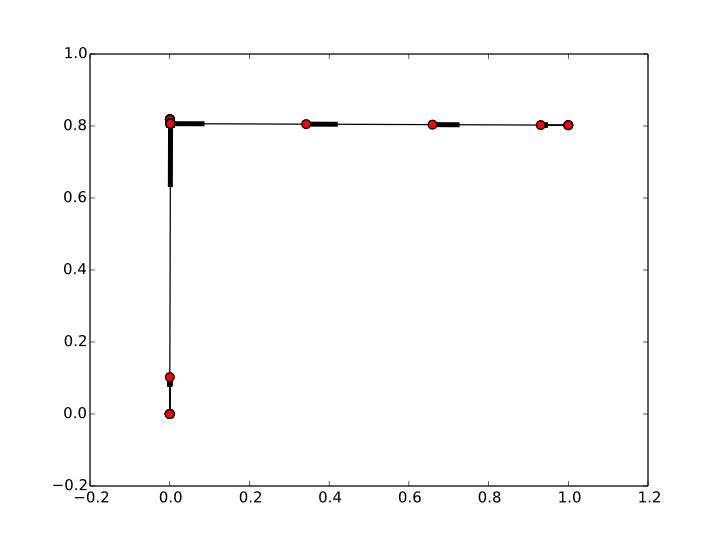
\includegraphics[scale=0.8]{./img/links.png}
    \caption{Simplified Links of our Established Network}
    \label{fig:links}
\end{figure}

If we look at the entire expanded network we see a similar picture. Our users are clustered around one main user, and it is obvious that the network has one focal point, however when examined closely it becomes apparent that some users have no connections to our main user and instead point to just one sub-user instead.

\begin{figure}[ht]
    \centering
    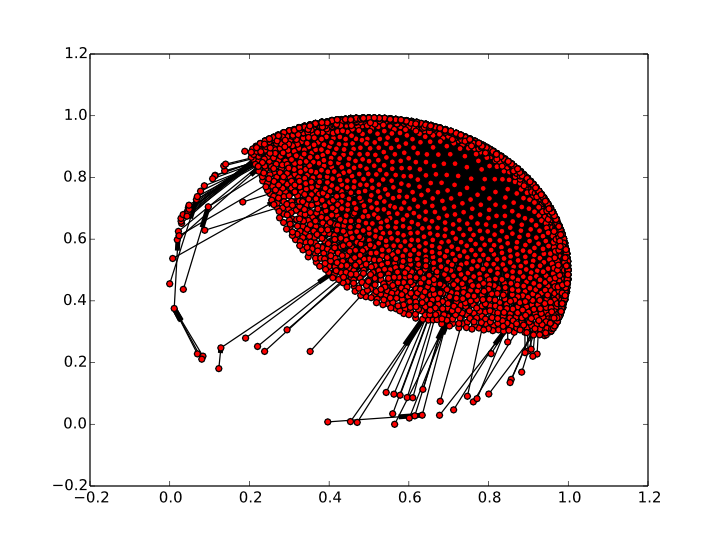
\includegraphics[scale=0.8]{./img/users.png}
    \caption{All Users of our Established Network}
    \label{fig:users}
\end{figure}

Given our results these networks make intuitive sense; we have one user that is focused upon, and everyone else is of little to no importance. When looking at Twitter's population this result begins to hold true for a large portion of Twitter users. Most users are either fairly passive or of too little consequence to be highlighted.
